% !TEX root = mythesis.tex



%==============================================================================
\chapter{Theoretical concepts}
\label{sec:theory}
%==============================================================================

%------------------------------------------------------------------------------
\section{The Standard Model}%
\label{sec:theory:standardmodel}
%------------------------------------------------------------------------------
The Standard Model (SM) of particle physics was developed in the late 1970s to combine all our current understandings of fundamental particles and forces. The SM is a quantum field theory which is described by Lagrangian dynamics. It postulates that all the matter in the Universe is made up of fundamental elementary particles called fermions that interact via particle fields mediated by gauge bosons.~\cite{thomson} 

The SM is the theoretical framework used in particle physics to describe and predict the interactions of particles. Some of the predictions made by the SM have been verified to very high accuracy by the experiments. This section outlines the ingredient of the SM and their interactions and provides a brief overview of the Higgs mechanism responsible for the electroweak symmetry breaking of the SM.

%------------------------------------------------------------------------------
\subsection{Particle content}%
\label{sec:theory:standardmodel:particle}
%------------------------------------------------------------------------------
In the Standard Model, fundamental particles are described as the excitation of quantum fields. The fundamental particles are divided into two groups based on a quantum number which represents their intrinsic angular momentum, known as spin. 

The matter is composed of half-integer spin particles called fermions which are constrained by the Pauli exclusion principle. The interactions between the fermions are mediated by integer spin particles called bosons. The energy distribution of bosons is described by the Bose-Einstein statistics~\cite{thomson}. The bosons are responsible for the three interactions described within the SM: the strong interaction, the weak interaction and electromagnetism, which are described in detail in the next sections. 

The energy distribution of fermions is described by the Fermi-Dirac statistics~\cite{thomson}. The fermions are further divided based on their sensitivity to the strong interaction. Fermions that are sensitive to the strong interaction are called quarks; otherwise, they fall into the category known as leptons. There are six types of quarks and leptons each, which are arranged in the form of generations in the SM. First-generation fermions include \Pup, \Pdown, \Pelectron and \Pnue. Second-generation fermions include \Pcharm, \Pstrange, \Pmuon and \Pnum. Third-generation fermions include \Ptop, \Pbottom, $\Ptau^{-}$ and \Pnut. The mass of the particles increases as one goes from first- to third-generation. Fig.\ \ref{fig:theory:standardmodel} shows all the fundamental particles on the left side and the force carriers on the right side. All six quarks are shown in purple and leptons in green. The SM also postulates a fundamental scalar boson responsible for the electroweak symmetry breaking within the SM, known as the Higgs boson as shown in yellow. Some elementary properties of these particles like their masses, electric charge and spin are also shown in the picture. The experimental evidence predicts the restriction on the number of generations of the lepton family to be three, but as far as concerned, there is no such restriction on the quark family.

The negative energy solutions of the Dirac equation predict the existence of the antiparticles~\cite{thomson}. So, all the 12 fermions have their antiparticles associated with them which exhibits precisely
the similar properties but carries an opposite charge of their corresponding particles.

\begin{figure}[hbt!]
	\centering
	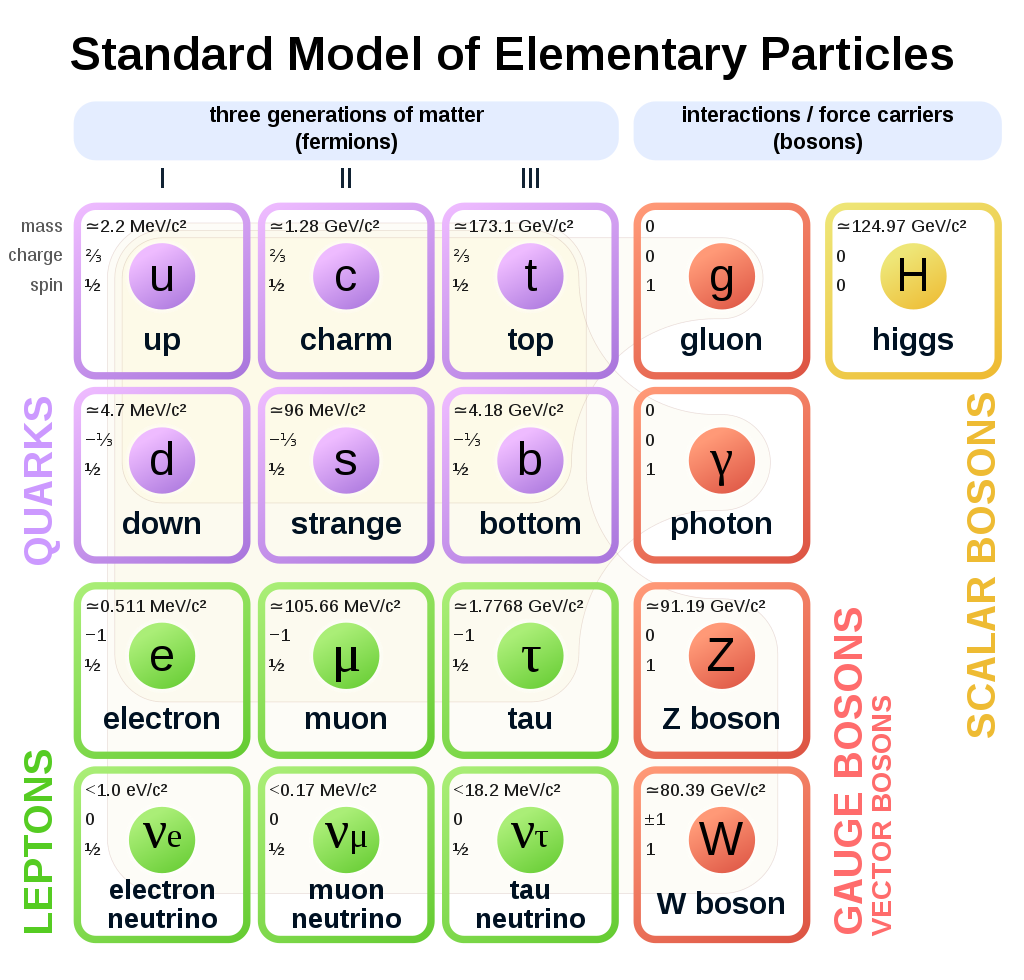
\includegraphics[width=0.85\linewidth]{standardmodel}
	\caption{Overview of all the ingredients of the Standard Model which constitutes all the fermions and the gauge bosons. Elementary properties like mass, electric charge and spin of all the particles are also shown in the image.~\cite{standardmodelpicture}}
	\label{fig:theory:standardmodel}
\end{figure}



%------------------------------------------------------------------------------
\subsection{Gauge groups}%
\label{sec:theory:standardmodel:gauge}
%------------------------------------------------------------------------------
The Standard Model is formed from the combination of three different local symmetry groups which can be written as:
\begin{equation}
	\text{SU(3)}_{\text{c}} \times \text{SU(2)}_{\text{L}} \times \text{U(1)}_{\text{Y}}
\end{equation}
where SU(3)$_{\text{c}}$ symmetry group is generated by the colour charge associated with the strong interaction, described in section \ref{sec:theory:standardmodel:strong}. The SU(2)$_{\text{L}} \times$ U(1)$_{\text{Y}}$ symmetry groups represent the left-handed isospin and hypercharge symmetries within the SM, which are generated by the unified electroweak interaction, described in section \ref{sec:theory:standardmodel:weak}. 

These local symmetries are applied to the SM Lagrangian ($\mathcal{L}_{\text{SM}}$) which correspond to local gauge invariance. The SM Lagrangian can be written as~\cite{halzen}:

\begin{equation}
	\mathcal{L}_{\text{SM}} = \mathcal{L}_{\text{Boson}} + \mathcal{L}_{\text{Fermion}} + \mathcal{L}_{\text{Yukawa}} + \mathcal{L}_{\text{Higgs}}
\end{equation}
where $\mathcal{L}_{\text{Boson}}$ + $\mathcal{L}_{\text{Fermion}}$ represents the kinetic energies, electroweak interaction and self-interaction of fermions and bosons. $\mathcal{L}_{\text{Yukawa}}$ is a term from Yukawa coupling which gives mass to the particles. $\mathcal{L}_{\text{Higgs}}$ describes the spontaneous symmetry breaking by Higgs field.

%------------------------------------------------------------------------------
\subsection{Electromagnetic Interaction}%
\label{sec:theory:standardmodel:em}
%------------------------------------------------------------------------------
The electromagnetic interaction (EM) is well described by one of the Quantum Field Theory (QFT), known as Quantum electrodynamics (QED). It is based on the $\text{U(1)}_{\text{Y}}$ gauge group which represents the interaction between the charged fermions and a massless gauge boson known as a photon. Photon is a vector gauge boson which acts as a force carrier of the EM interaction. Only neutrinos (and their antiparticles) do not interact via the EM interaction because they are electrically neutral. $\text{U(1)}_{\text{Y}}$ is Abelian in nature which means it is a commuting gauge group that does not allow any self-interaction terms for the photon field.

The QED Lagrangian for a charged fermion ($\psi$) of mass $m$ can be written as:
\begin{equation}
	\mathcal{L}_{\text{QED}} = \bar{\psi}(i\textbf{D}_{\text{QED}} - m)\psi - \frac{1}{4}F_{\mu\nu}F^{\mu\nu}
\end{equation}
where $F$ is the electric field tensor which can be expressed in terms of the photon vector field by $F^{\mu\nu} = \partial^{\mu}A^{\nu} - \partial^{\nu}A^{\mu}$ and $\textbf{D}_{\text{QED}}$ is a covariant derivative which also depends the photon vector field $A$.~\cite{halzen}

%------------------------------------------------------------------------------
\subsection{Strong Interaction}%
\label{sec:theory:standardmodel:strong}
%------------------------------------------------------------------------------
The strong interaction is described by a theory called the Quantum Chromodynamics (QCD). It explains the interaction between partons which include quarks and gluons. Gluons are vector gauge boson which mediates the strong interaction. Like electric charge in the QED, QCD also introduces a new type of property called colour charge. There are three different types of colour charges: red, blue and green. So, all the six types of quarks and their antiparticles can be represented as colour triplets. Particles carrying a colour charge can feel the effects of the strong interaction. The strong force is described by the $\text{SU(3)}_{\text{c}}$, which is a non-Abelian gauge group that means it allows the self-interaction terms for the gluons. Due to the non-abelian nature of the force, it is more complex than the EM force, and give rise to eight different coloured gluons.~\cite{halzen}

The strong interaction is the strongest among all the three interactions described in the SM. One of the consequences of the QCD is the process of hadronisation which means that partons can only exist in bound colour neutral states called hadrons, such as the proton. The strength of the coupling constant of the strong interaction increases with the distance between the coloured particles due to the gluon self-interaction. If one tries to separate the two quarks within a hadron, a large amount of energy is required, and at some point it spontaneously produces into a quark-antiquark pair, turning the initial hadron into a pair of hadrons instead of producing an isolated coloured quark. This phenomenon is known as \textit{colour confinement}. The strength of the coupling constant of the strong interaction is low at small distances, so the quarks exist freely inside the hadrons. This feature of the QCD is known as \textit{asymptotic freedom}.~\cite{thomson}

There are two groups of hadrons: baryons and mesons. Baryons are made up of three quarks or antiquarks while mesons are made from a quark-antiquark pair. The effects of the hadronisation can be seen as clusters in the particle detectors, which are further reconstructed as Jets. Jets are the important physics object for this thesis and are discussed in detail in Chapter \ref{sec:jetsandtaggers}.

The QCD Lagrangian for a coloured charged fermion ($\psi$) of mass $m$ can be written as:
\begin{equation}
\mathcal{L}_{\text{QCD}} = \bar{\psi}_{j}(i\gamma^{\mu}\textbf{D}_{\text{QED,}\mu} - m_{j})\psi_{j} - \frac{1}{4}G_{\mu\nu}^{\alpha}G^{\mu\nu}_{\alpha}
\end{equation}
where $G_{\mu\nu}^{\alpha}$ is a gluon field tensor which includes the additional self-interaction term of the gluon vector fields and $\alpha$ is denoted as the eight coloured gluons. $\textbf{D}_{\text{QED,}\mu}$ is a covariant derivative which can be expressed in terms of the gluon gauge field $A_{\mu}^{\alpha}$ and the strong coupling constant $\alpha_{\text{s}}$. Index $j$ is indicated as all the coloured flavours of the quarks.~\cite{halzen}

%------------------------------------------------------------------------------
\subsection{Weak Interaction and Electroweak unification}%
\label{sec:theory:standardmodel:weak}
%------------------------------------------------------------------------------
The weak interaction is described by a theory called the Quantum Flavourdynamics (QFD). It explains the interaction between particles that is responsible for the radioactive decay of atoms. The Lagrangian of the weak interaction is constructed only from left-handed doublets in the $\text{SU(2)}_{\text{L}}$ gauge group since right-handed particles in the SM appeared as singlets and are not affected by the weak force. The weak force is better understood in terms of the Electroweak Theory (EWT).~\cite{halzen}


In the Standard Model, the electromagnetic and weak interactions are unified at an energy of electroweak scale and described by the electroweak theory proposed by Glashow, Salam and Weinberg. The electroweak interaction is described by $\text{SU(2)}_{\text{L}} \times \text{U(1)}_{\text{Y}}$ gauge group where L denotes the SU(2) doublet and singlet representation of left-handed particles and Y is denoted as the weak hypercharge, given as Y = Q - $I_{3}$. Here, $I_{3}$ is the third component of the weak isospin.

The electroweak Lagrangian for fermions can be written as:
\begin{equation}
\mathcal{L}_{\text{EW}} = \bar{\psi}_{f}i\gamma^{\mu}\textbf{D}_{\text{EW,}\mu}\psi_{f}
\end{equation}
where the fermionic fields $\psi_{f}$ are organised in $\text{SU(2)}_{\text{L}}$ doublets and singlet, as shown below:

\begin{equation}
	\psi_{\text{lepton}} = \begin{pmatrix} \Pnue \\ e \end{pmatrix}_{L}, \begin{pmatrix} \Pnum \\ \mu \end{pmatrix}_{L}, \begin{pmatrix} \Pnut \\ \tau \end{pmatrix}_{L}, e_{R}, \mu_{R}, \tau_{R}
\end{equation}

\begin{equation}
\psi_{\text{quark}} = \begin{pmatrix} u \\ d \end{pmatrix}_{L}, \begin{pmatrix} c \\ s \end{pmatrix}_{L}, \begin{pmatrix} t \\ b \end{pmatrix}_{L}, u_{R}, d_{R}, c_{R}, s_{R}, t_{R}, b_{R}
\end{equation}


The electroweak theory is a parity-violating theory, so right-handed neutrinos are omitted in the SM. There are four vector fields which contribute to the electroweak interaction. A linear combination of $W^{1}_{\mu}$ and $W^{2}_{\mu}$ describes the two charged $W$ bosons, as shown below:
\begin{equation}
	W^{\pm}_{\mu} = \frac{1}{\sqrt{2}}(W^{1}_{\mu} \mp iW^{2}_{\mu})
\end{equation}

And the linear combination of $W^{3}_{\mu}$ and $B_{\mu}$ represents the two neutral bosons, the $Z$ boson and the photon as shown below:
\begin{align}
	A_{\mu} = \sin\theta_{W}W^{3}_{\mu} + \cos\theta_{W}B_{\mu} \\
	Z_{\mu} = \cos\theta_{W}W^{3}_{\mu} - \sin\theta_{W}B_{\mu}
\end{align}
where $\theta_{W}$ is called the Weinberg angle and is given by $\tan\theta_{W} = \frac{g}{g'}$ where $g$ and $g'$ are the gauge coupling constants.

%------------------------------------------------------------------------------
\subsection{Higgs mechanism}%
\label{sec:theory:standardmodel:higgs}
%------------------------------------------------------------------------------
The addition of mass terms to the Lagrangians shown before would break the gauge symmetry of the model, so a different process is required for particles to become massive. The process which describes how these bosons acquire their mass, without breaking the gauge invariance of the SM, is called the Higgs mechanism. The Higgs mechanism introduces \textit{spontaneous symmetry breaking} of the $\text{SU(2)}_{\text{L}} \times \text{U(1)}_{\text{Y}}$ gauge group by adding a new complex scalar doublet field, called the Higgs field.~\cite{halzen} 

Let us consider a weak isospin doublet of two complex fields ($\Phi$):
\begin{equation}
	\Phi = \begin{pmatrix} \phi^{+} \\ \phi^{o} \end{pmatrix}
\end{equation}
Then the potential $\mathcal{U}(\Phi))$ given by the complex field can be written as:
\begin{equation}
	\mathcal{U}(\Phi)) = \mu^{2}(\Phi^{*}\Phi) + \lambda(\Phi^{*}\Phi)^{2}
\end{equation}

Only solution with $\lambda>0$ and $\mu^{2}<0$ is considered so that the energy of the potential is bounded below and leads to a non-unique ground state energy. The minimum of this potential is not at the zero value of the field and is given by $v = \sqrt{\mu^{2}/\lambda}$. Now the Lagrangian can be written as~\cite{halzen}:
\begin{equation}
	\mathcal{L}_{Higgs} = |\textbf{D}_{\mu}\Phi|^{2} - \mu^{2}(\Phi^{*}\Phi) - \lambda(\Phi^{*}\Phi)^{2}
\end{equation}
By expanding the Lagrangian around the vacuum expectation value ($vev$), a mass term is introduced for the vector bosons. The masses of the bosons predicted by this mechanism are related in the following way:

\begin{align}
	m_{\text{H}} = \sqrt{2}\mu \\
	m_{\text{W}^{\pm}} = \frac{1}{2}vg \\
	m_{\text{Z}} = \frac{1}{2}v\sqrt{g^{2} + g'^{2}} \\
	\cos\theta_{W} = \frac{m_{\text{W}}}{m_{\text{Z}}}
\end{align}

Fermions also acquire mass through the Higgs mechanism by interactions between the fermionic and Higgs scalar fields, called Yukawa couplings.~\cite{halzen}




















%------------------------------------------------------------------------------
\section{The Standard Model}%
\label{sec:theory:standardmodel}
%------------------------------------------------------------------------------
The Standard Model is the most reliable attempt by mankind to understand the nature of the Universe. It provides a unified picture of the behaviour of the fundamental particles.  The key constituents of this remarkable theory are the elementary particles and the interactions between them as shown in Fig. \ref{fig:theory:standardmodel}. Remarkably, it has been developed out over the last few decades through a lot of experiments and various theories to unite all the gained information into one theory. This section gives a brief description of the elementary particles and their interaction with the forces.


\begin{figure}[hbt!]
	\centering
	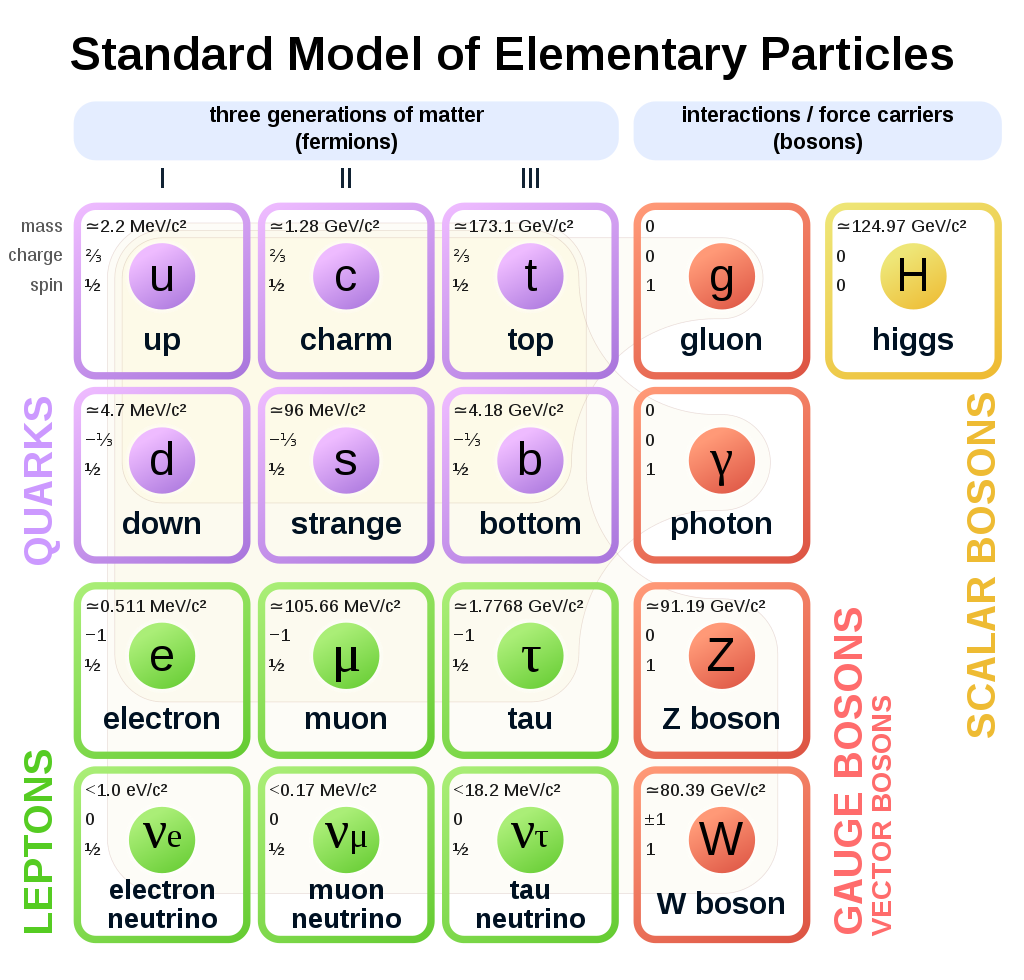
\includegraphics[width=0.85\linewidth]{standardmodel.pdf}
	\caption{Overview of all the particles of the Standard Model which constitutes elementary particles and the force carriers along with their mass, electric charge and spin. The figure is taken from \cite{standardmodelpicture}.}
	\label{fig:theory:standardmodel}
\end{figure}


%------------------------------------------------------------------------------
\subsection{Fundamental particles}%
\label{sec:theory:standardmodel:fundamentalparticles}\index{fundamentalparticles}
%------------------------------------------------------------------------------
Particles are divided into different subgroups, where the primary classification is fermions or bosons:

%------------------------------------------------------------------------------
\subsubsection{Fermions}%
\label{sec:theory:standardmodel:fundamentalparticles:fermions}\index{fermions}
%------------------------------------------------------------------------------

Fermions are defined as the particles with half-integer spin or \enquote{intrinsic angular momentum} and therefore are constrained by the Pauli exclusion principle. The energy distribution of fermions is described by the Fermi-Dirac statistics \cite{thomson}. They are also regarded as the building blocks of everyday matter. A fermion can be an elementary particle, such as the electron, or it can be a composite particle, such as the proton. They are further classified into quarks and leptons depending upon their interaction with the strong force.


\begin{enumerate}
	\item \textbf{Quarks (\Pquark)} \label{sec:theory:standardmodel:fundamentalparticles:fermion:quarks}\index{quarks}
	\\ All the fermions feel the weak force and undergo weak interaction, but quarks also interact via the strong interaction. So, their properties are different from leptons. Quarks carry the QCD equivalent of electric charge, called $colour$ $charge$ and are highlighted in purple in Fig. \ref{fig:theory:standardmodel}. They are further divided into three generations depending on their masses:
	
	\begin{itemize}
		\item \textbf{First-generation quarks:} up (\Pup) and down (\Pdown) quarks are the members of the first-generation of quarks family having masses of \SI[per-mode=symbol]{2.2}{\mega\electronvolt\per\clight^2} and \SI[per-mode=symbol]{4.7}{\mega\electronvolt\per\clight^2} respectively. They have a tiny mass as compared to the other generation quarks. They interact weakly, strongly and electromagnetically, carrying an electric charge of $+\frac{2}{3}$ and $-\frac{1}{3}$ respectively. In nature, the up and down quarks form protons (\Pup \Pup \Pdown) and neutrons (\Pup \Pdown \Pdown).
		
		\item \textbf{Second-generation quarks:} charm (\Pcharm) and strange (\Pstrange) quarks are the members of the second-generation of quarks family having masses of \SI[per-mode=symbol]{1.28}{\giga\electronvolt\per\clight^2} and \SI[per-mode=symbol]{96}{\mega\electronvolt\per\clight^2} respectively. They are massive as compared to the first-generation quarks but lighter than third-generation quarks. They interact weakly, strongly and electromagnetically, carrying an electric charge of $+\frac{2}{3}$ and $-\frac{1}{3}$ respectively. Second-generation quarks are found in hadrons, which are subatomic particles made up of quarks. For example, \PJpsi meson is a bound state of charm quark with their antiparticle (\Pcharm\APcharm), whereas \PDs mesons contain a charm quark and a strange quark (\Pcharm\Pstrange).
		
		\item \textbf{Third-generation quarks:} top (\Ptop) and bottom (\Pbottom) are the members of the third-generation of quarks family having masses of \SI[per-mode=symbol]{173}{\giga\electronvolt\per\clight^2} and \SI[per-mode=symbol]{4.18}{\giga\electronvolt\per\clight^2} respectively. They are massive among all the generations of quarks family. They interact weakly, strongly and electromagnetically, carrying an electric charge of $+\frac{2}{3}$ and $-\frac{1}{3}$ respectively. Due to such a large mass of top quark, the value of Yukawa coupling is very close to one which makes the top quark an interesting probe into physics issues that cannot be explained by the Standard Model. Top quark also has a very short lifetime which leads to a decay of the quark before it can undergo hadronisation, which is the processes of other generation quarks combining to form hadrons.
	\end{itemize}
	
	\item \textbf{Leptons (\Plepton)} \label{sec:theory:standardmodel:fundamentalparticles:fermion:leptons}\index{leptons}
	\\ Leptons do not undergo strong interaction and are highlighted in green in Fig. \ref{fig:theory:standardmodel}. Like quarks, leptons are also grouped into three generations depending upon their masses which increases as we move from first to the third generation. Theory and experimental evidences predict the restriction on the number of generations of the lepton family to be three \cite{thomson}. So in general, there are six types of leptons, also known as flavours. Besides this, leptons are additionally classified into charged leptons and neutral leptons depending upon their electric charge. 
	
	\begin{enumerate}
		\item \textbf{Charged leptons (\Pleptonpm):} It comprises of an electron (\Pelectron), muon (\Pmuon) and tau (\Ptau) carrying a negative unit charge. They can interact either via electromagnetic interaction or by the weak interaction. Electrons combine with other particles to form various composite particles like they form an atom along with proton and neutron. The more massive muons and taus decay into electrons and neutrinos through a process of particle decay. Thus electrons are stable and the most common charged lepton in the Universe. Muons and taus are produced in high energy collisions involving cosmic rays as well as the particle accelerator.
		
		\item \textbf{Neutral leptons (\Plepton):} Often known as \enquote{$neutrinos$} which are charged lepton partners, comprises of electron neutrino (\Pnue), muon neutrino (\Pnum) and tau neutrino (\Pnut). Neutrinos do not carry any electric charge and were long believed to be massless, but it is now known that they carry a very little mass. Due to which, they only interact via the weak interaction. Neutrinos typically pass through matter unimpeded and undetected \cite{neutrino}. They are often produced along with their corresponding charged leptons by the weak interaction. They are also produced in radioactive decays such as beta decay of atomic nuclei or hadrons.
	\end{enumerate}
	
	\item \textbf{Antiparticles} \label{sec:theory:standardmodel:fundamentalparticles:fermion:antiparticles}\index{antiparticles}
	\\The negative energy solutions of the Dirac equation predict the existence of the antiparticles \cite{thomson}. So, all the \num{12} fermions have their antiparticles associated with them which exhibits precisely the similar properties and mass but carrying an opposite charge of their corresponding particles. First-generation antiparticles include anti-up (\APup), anti-down (\APdown), positron (\APelectron) and anti-electron neutrino (\APnue). Second-generation antiparticles include anti-charm (\APcharm), anti-strange (\APstrange), anti-muon (\APmuon) and anti-muon neutrino (\APnum). Third-generation antiparticles include anti-top (\APtop), anti-bottom (\APbottom), anti-tau (\APtauon) and anti-tau neutrino (\APnut).
	
	Antiparticles cannot be observed easily in nature except the positron (\APelectron), which can be found in nature for a short period of time by so-called $\beta^{+}$ radiation in nuclear decays. Also, electron antineutrino (\APnue) can be detected indirectly in $\beta^{+}$ nuclear decay \cite{thesis:tanja}.
	
\end{enumerate}

%------------------------------------------------------------------------------
\subsubsection{Bosons}%
\label{sec:theory:standardmodel:fundamentalparticles:bosons}\index{bosons}
%------------------------------------------------------------------------------

Bosons are defined as the particles with integer spin or "intrinsic angular momentum" and therefore are not constrained by the Pauli exclusion principle. The energy distribution of bosons is described by the Bose-Einstein statistics \cite{thomson}. They are also regarded as the force carrier which holds the building blocks of everyday matter and are highlighted in red in Fig. \ref{fig:theory:standardmodel}. They are further classified into four different types depending upon the strength of the interaction.

\begin{itemize}
	\item \textbf{Gluon (\Pgluon):} is the vector gauge boson which is massless and electrically neutral but carries the colour charge. Gluons are the force carrier of the strong interaction, which are associated mainly with all the quarks since they carry the colour charge. Unlike photon, which only mediates the electromagnetic interaction but does not carry any electric charge, gluons also participate in the strong interaction in addition to mediating it, making Quantum Chromodynamics (QCD) significantly more challenging to probe than Quantum Electrodynamics (QED). The strength of the strong interaction is extreme as compared to the other forces. Gluons are responsible for the conservation of the colour charge.
	
	\item \textbf{Photon (\Pphoton):} is the vector gauge boson which is massless and electrically neutral. Photons are the force carrier of the electromagnetic interaction, which are associated mainly with all the fermions except neutrinos and antineutrinos since they are electrically charged neutral. The strength of the electromagnetic interaction is less than strong interaction. They cannot change the flavour of the fermions, and responsible for the conservation of the electric charge.
	
	\item \textbf{W boson (\PWpm) and Z boson (\PZzero):} are the vector gauge bosons having masses of \SI[per-mode=symbol]{80}{\giga\electronvolt\per\clight^2} and \SI[per-mode=symbol]{91}{\giga\electronvolt\per\clight^2} respectively.  W boson has either positive or negative unit charge depending upon the sign of the isospin, whereas Z boson is electrically neutral. The W and Z boson together are known as the carrier of the weak interaction, which is associated with all the fermions. All three of these particles have finite masses and harder to exchange \cite{thesis:tanja}; therefore, they are very short-lived. The weak force is virtually as strong as the electromagnetic force, but it seems weak because its impact is restricted by the large mass of the W and Z bosons. Their mass limits the range of the weak force and vanishes completely beyond the radius of a single proton. W boson can change the flavour as well as the electric charge of the fermion, whereas Z boson can only change the flavour of the fermion.
	
	\item \textbf{Higgs boson (\PHiggs):} is the scalar gauge boson having the mass of \SI[per-mode=symbol]{125}{\giga\electronvolt\per\clight^2} and is highlighted in yellow in Fig. \ref{fig:theory:standardmodel}. It is electrically neutral as well as colour neutral. The Higgs is not associated with a force but rather to the mechanism known as \enquote{Higgs mechanism} which gives mass to the fermions. Therefore it couples to the mass of the fermions. The Higgs mechanism proposes the existence of the Higgs boson which was confirmed in 2012 by the ATLAS and CMS collaborations in the LHC at CERN \cite{higgsatlas,higgscms}.
	
\end{itemize}



%%% Local Variables: 
%%% mode: latex
%%% TeX-master: "mythesis"
%%% End: 
